\documentclass{article}

% if you need to pass options to natbib, use, e.g.:
% \PassOptionsToPackage{numbers, compress}{natbib}
% before loading rl_project.

% to compile a camera-ready version, add the [final] option, e.g.:
 \usepackage[final]{dissertation}

% to avoid loading the natbib package, add option nonatbib:
% \usepackage[nonatbib]{rl_project}

\usepackage[utf8]{inputenc} % allow utf-8 input
\usepackage[T1]{fontenc}    % use 8-bit T1 fonts
\usepackage{hyperref}       % hyperlinks
\usepackage{url}            % simple URL typesetting
\usepackage{booktabs}       % professional-quality tables
\usepackage{amsfonts}       % blackboard math symbols
\usepackage{nicefrac}       % compact symbols for 1/2, etc.
\usepackage{microtype}      % microtypography
\usepackage{graphicx}
\usepackage{natbib}
\usepackage{amsfonts}
\usepackage{amsmath}
\usepackage{pgfgantt}


\title{A Comparative Analysis of the Performance of Emulated Ternary vs Binary Logic Systems \\ [1ex] \large Project Proposal}

\author{
  Thomas Timmons \\
  Bachelor of Science in Computer Science \\
  The University of Bath \\
  November 8, 2024 \\
  \texttt{tlt33@bath.ac.uk} \\
  %% examples of more authors
  %% \And
  %% Coauthor \\
  %% Affiliation \\
  %% Address \\
  %% \texttt{email} \\
}

\begin{document}

\maketitle

% \section{Overview}
% An investigation into ternary logic in comparison to binary logic where theoretical components are implemented in an 
% emulator which can be directly compared against a binary counterpart. Measuring the impacts of the theoretical 
% advantages of ternary in a practical manner will predict it's useability given that the circuits can be implemented on a 
% more exotic machine.

\section{Problem Description}

% \subsection{Motivation}

% insert a figure here
In 1965, Gordon Moore, made an observation that density of transistors within integrated circuits
grow exponentially over time and predicted that it would double every two years. 
This later became known as Moore's Law and almost 60 years later, this still holds true.

\begin{figure}[h]
  \centering
  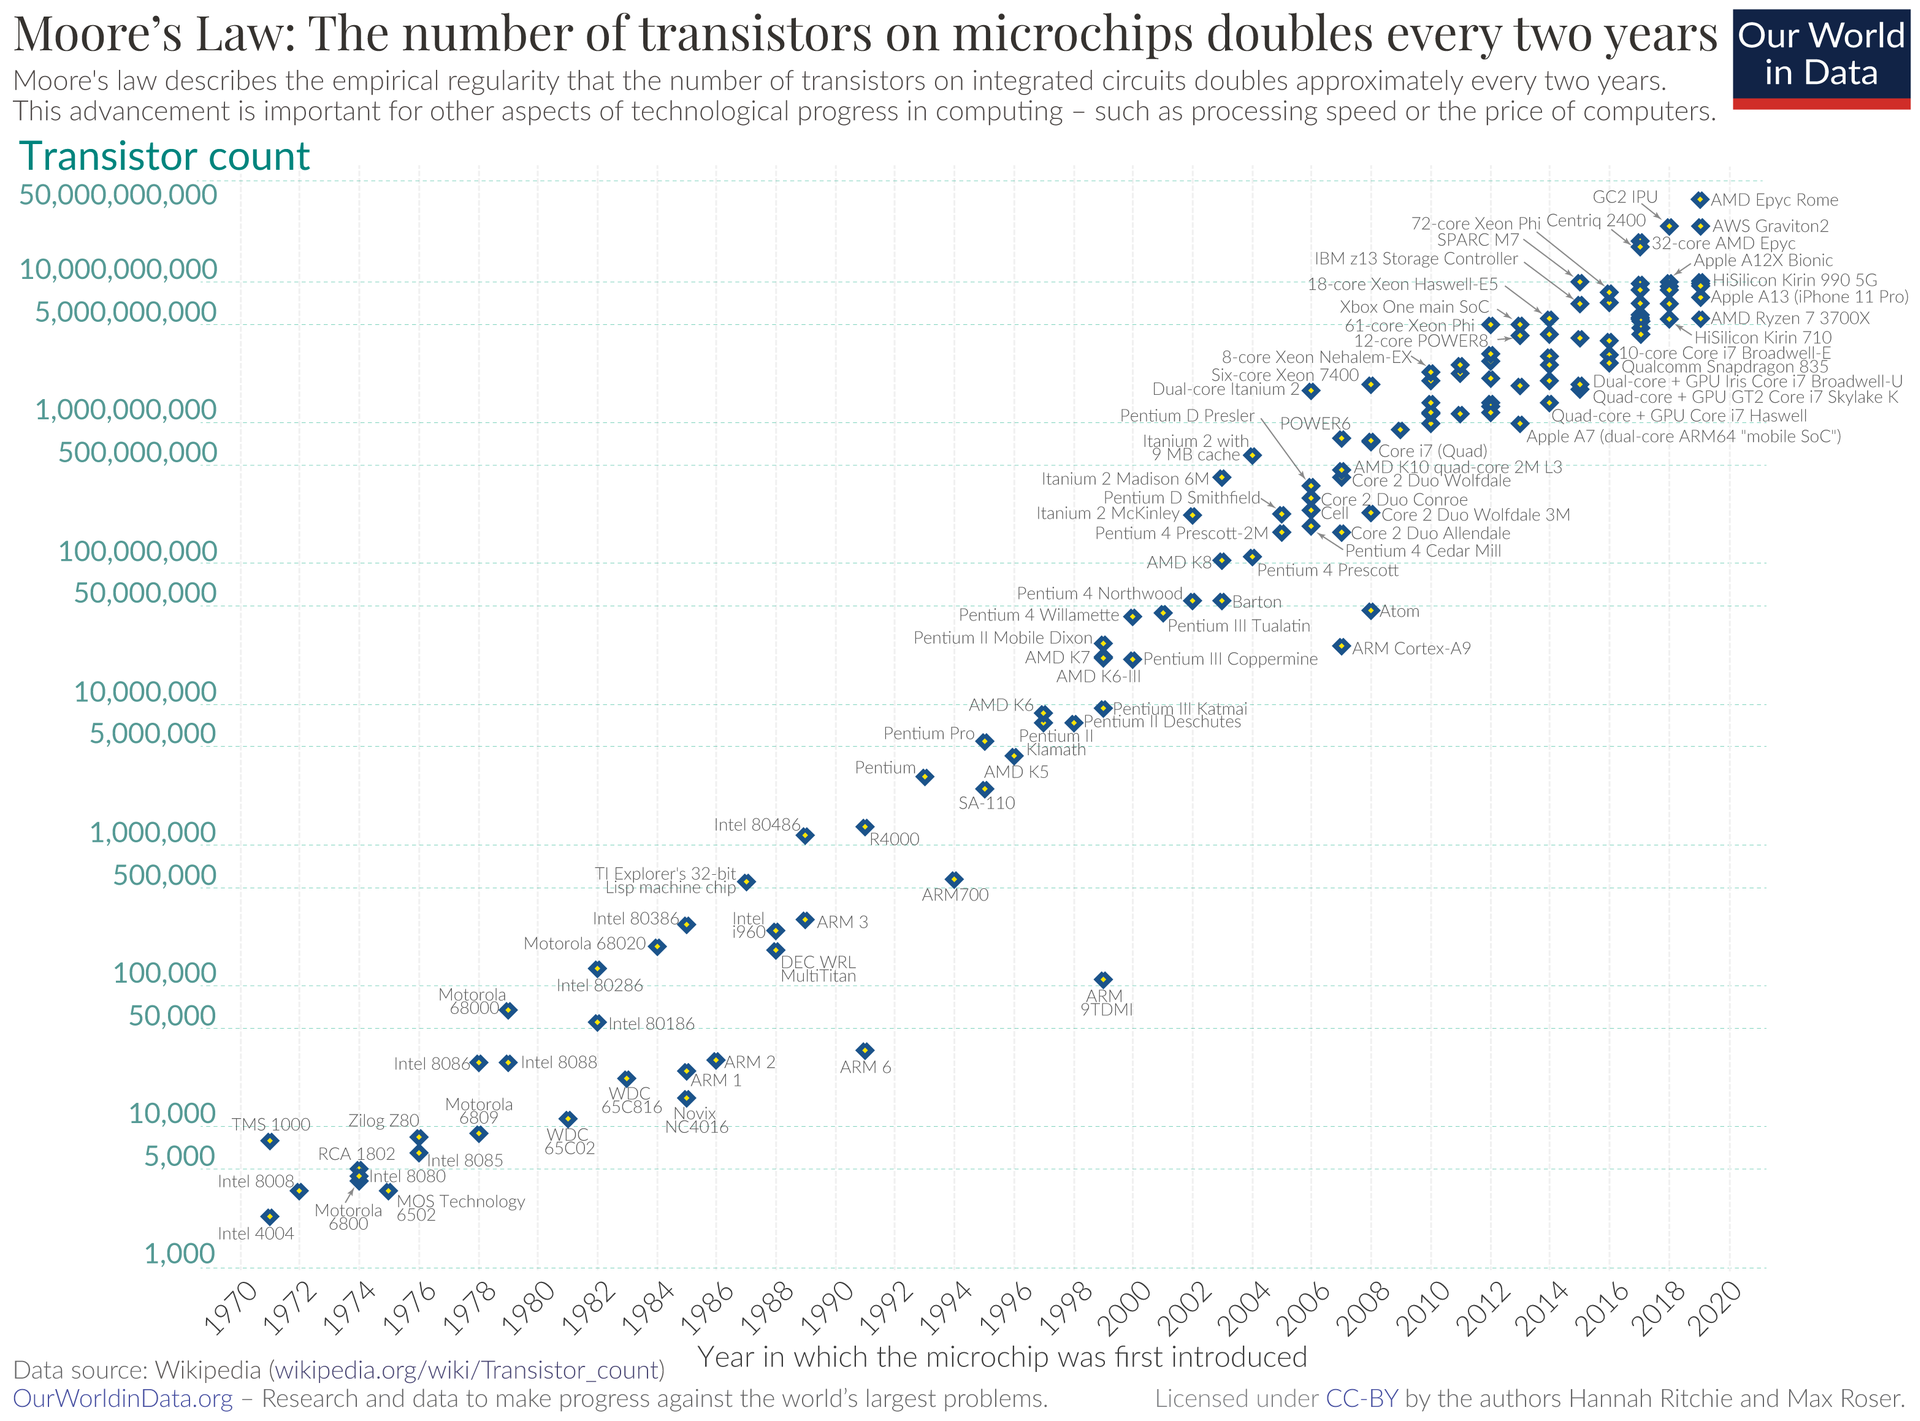
\includegraphics[width=0.5\textwidth]{figures/moores_law.png}
  \caption{Moore's Law}
  \label{fig:moores_law}
\end{figure}

The implication of Moore's law is that the performance of digital systems has also increased exponentially over time.
\citep{moore1965cramming}
Many of the devices we use today, reap the benefits of this increase in performance. Smaller and faster computers
have allowed for improvement in industries such as health care, education, transportation and along with many others 
that have helped create a higher standard of living for many people around the world.

However, researchers have begun to question the sustainability of Moore's Law as the size of transistors approach the
atomic scale and the physical limits of Moore's law should be reached at some point in the 2020's.
\citep{zhou2020quantum}

Even Moore himself was quoted in 2006 saying "...the fact that materials are made of atoms is the fundamental limitation
and it's not that far away...We're pushing up against some fairly fundamental limits so one of these days we're going to 
have to have to stop making things smaller".
\citep{moore2006interview}

This has led to the exploration of alternative computing paradigms such as quantum computing.

\subsection{Ternary Algebra}

To represent any given range of values $N$, with the radix of value is given by $R$ and the necessary number of digits 
required is $d$ (rounded upwards to the nearest integer):

\begin{equation}
  N = R^{d}
\end{equation}

The cost or complexity of the system $C$ is directly proportional to the capacity of the digits $(R \cdot d)$.
Therefore for some constants $k$ and $\log N$:
\citep{hurst1984mvl}

\begin{equation}
  C = k(R \cdot d) = k(R \cdot \frac{\log N}{\log R}) = k \log N (\frac{R}{\log R})
\end{equation}

Minimising this cost $C$ can be done by differentiating with respect to $R$ and setting the result to $0$:

\begin{equation}
  \frac{\partial C}{\partial R} = 
  k\log N\cdot\frac{d}{dR}\left[\frac{R}{\log R}\right] = 
  k\log N\cdot \frac{\log R -1}{(\log R)^2} = 0
\end{equation}

After removing constants $\log R = 1$ and solving for $R = e = 2.718$. Since as stated above, the radix $R$ must be an 
integer then we are left with $R = 3$. Therefore, the ternary logic system is the most efficient.
\citep{jaber2020mvl}

In binary logic the binary set of values is $\mathbb{B} = \{0, 1\}$ while the symbol $\mathbb{T}$ will be used to denote 
the ternary set. There exists a variety of valid ternary sets with the most natural being an extension of binary called
unbalanced ternary where $\mathbb{T} = \{0, 1, 2\}$. Unknown state ternary where $\mathbb{T} = \{T, ?, F\}$.

In this paper we will be using balanced ternary where $\mathbb{T} = \{-, 0, +\}$. This will allow operations on 
negative and positive numbers without having to use the ternary equivalent of two's complement.

\subsection{Aims}

Researchers have attempted to investigate this field using two distinct approaches. One from a more theoretical perspective
or looking at the theoretical gains of ternary logic while others taking a more practical approach. Ternary test benches
have been created in order to attempt to validate the theoretical performance gains.

However, the underlying implementations of the basic ternary logic is underpinned by Complementary Metal Oxide 
Semiconductor (CMOS) along with PMOS and MNOS.

For this project I propose several theoretical gates whose logic can be implemented in hardware that have the same relative 
speed to their binary counterparts. More formally we assume the following is true in regards to propagation delay:

\begin{equation}
\begin{aligned}
  AND &\equiv \mathbb{T}AND \\
  OR &\equiv \mathbb{T}OR \\
  NOT &\equiv \mathbb{T}NOT
\end{aligned}
\end{equation}

This will allow us to create a basic binary and ternary emulator whose performance will be directly comparable.

The aims for this project are too:
\begin{itemize}
  \item Collate research around how ternary logic can be implemented and the equivalence of a variety of operations across the two bases.
  \item Build two emulators with both binary and ternary logic respectively with an equivalent architecture.
  \item Practically test the theoretical benefits of ternary logic over it's binary counterparts.
\end{itemize}

\subsection{Objectives}

There are 3 main objectives that must be reached:
\begin{enumerate}
  \item Build a binary emulator with a very basic CPU architecture and simple instruction set.
  \item Build a ternary emulator with an equivalent CPU architecture and instruction set.
  \item Write a simple complier to create code to run on both machines.
\end{enumerate}

\section{Requirements Specification}

\subsection{Metrics}

The performance of various CPU's can be measured using the following criteria:

\begin{itemize}
  \item Power Consumption
  \item Cost
  \item Maximal Frequency
  \item Instructions Per Cycle (IPC)
  \item Architecture Efficiency
  \item Number of Cores
  \item Cache Size and Speed
  \item Thermal Efficiency
\end{itemize}

We will only be considering the maximal frequency for these systems as power consumption, cost and thermal efficiency 
are hard to deterministically measure within an emulator. The other possible metrics are discussed in the optimisations
section.

The maximal frequency, also know as clock speed, of a CPU represents the number of cycles it can execute per 
second, typically measured in Hertz in the order of GHz. 
However, we will be measuring the time taken for the signal to propagate through the circuit. This is determined by the longest path 
of the electric signal known as the critical path. Using our theoretical gates stated above (1) we can simply 
calculate the propagation time for any given circuit by the number of gates required to perform any given operation.

Time taken for delay in wires will not be taken into consideration.

All base gates will have an arbitrary unit for propagation time of 1 whereas more complex gates will have greater
propagation times.

\subsection{Optimisations}

Binary systems have had decades of research and optimisation over their ternary counterparts. The aim of this paper is 
not too optimise ternary circuits and will therefore not be implementing optimisations in either circuits 
as we are only concerned with the relative performance.

In reference to the criteria above, only the the architectural efficiency of the emulator will be considered as both 
will only have a single core with no cache.

\subsection{Requirements}

Below is a detailed set of requirements needed to meet the objectives set above and in turn fulfill the aims of the 
project. There will be categorised by the MoSCoW prioritisation method as shown below:

\begin{enumerate}
  \item \textbf{Must} - Non-negotiable requirement.
  \item \textbf{Should} - Important but not vital to the outcome.
  \item \textbf{Could} - Desirable but only to be done if their is extra time.
  \item \textbf{Won't} - Out of scope of the project due to time constraints.
\end{enumerate}

\subsubsection{Functional}

\begin{itemize}
  \item Both emulators \textbf{must} be built in Rust due to a lack of flexibility within emulating tools due to being 
  so closely tied to binary logic. 
  \item Both emulators \textbf{must} have an arithmetic and logic unit, control unit, program counter and 
  and registers within the CPU.
  \item Both emulators \textbf{must} have a comparable amount of memory although it does not need to be exact.
  \item Both emulators \textbf{must} be able to measure the propagation delay for any algorithm performed in the emulator.
  \item Both emulators \textbf{should} be able to handle floating point arithmetic.
  \item A testing workbench \textbf{must} be implemented in order to be able to record interactions with the emulator 
  simultaneously.
  \item Design and building a compiler \textbf{should} be implemented to allow for fast test cycle.
  \item Cache \textbf{won't} be implemented on either emulator as won't affect comparability.
  \item A system kernel \textbf{won't} be implemented on either emulator as it is outside of the scope of the project.
\end{itemize}

\subsubsection{Non-Functional}

\begin{itemize}
  \item A Literature, Technology and Data Survey \textbf{must} be completed by the 6th December 2024.
  \item A basic implementation of both emulators must be implemented for the demonstration of progress on the 
  17th February 2024.
  \item The project \textbf{must} be completed by the 2nd May 2025.
\end{itemize}

\textit{The above requirements are not fixed and are subject to change as the project progresses and develops.}

\section{Project Plan}

\subsection{Deliverable Deadlines}

\begin{center}
\begin{tabular}{ |c|c| }
  \hline
  Deliverable & Date \\
  \hline\hline
  Project Proposal & 08/11/24 \\
  Literature, Technology and Data Survey & 06/12/24 \\
  Demonstration of Progress & 17/02/25 \\
  Dissertation & 02/05/2025 \\
  \hline
\end{tabular}
\end{center}

\subsection{Initial Gantt Chart}

\begin{center}
\begin{tabular}{ |c|c|c|c| }
  \hline
  Task & Start Date & End Date & Effort (Hours) \\
  \hline\hline
  Project Proposal & 10/11/24 & 17/11/24 & 20 \\
  Literature, Technology and Data Survey & 18/11/24 & 29/11/24 & 20 \\
  Research and Design Basic Emulator & 30/11/24 & 15/01/25 & 60 \\
  Implement Binary Emulator in Rust & 7/12/24 & 30/01/24 & 75 \\
  Translate Binary Architecture into Ternary & 01/01/25 & 15/02/25 & 100 \\ 
  Implement Ternary Emulator in Rust & 15/01/25 & 30/02/25 & 40 \\
  Implement hardware specific circuits & 15/02/25 & 15/03/25 & 20 \\
  Evaluation & 15/03/25 & 01/04/25 & 40 \\
  Final Write-Up & 15/02/25 & 02/05/25 & 100 \\
  \hline
\end{tabular}
\end{center}

\begin{center}
\begin{ganttchart}[vgrid, hgrid]{1}{23}
  \gantttitle{Project Plan}{23} \\
  \gantttitlelist{46, 47, 48, 49, 50, 51, 52, 1, 2, 3, 4, 5, 6, 7, 8, 9, 10, 11, 12, 13, 14, 15, 16}{1} \\
\ganttbar{Project Proposal}{1}{1} \\
\ganttlinkedbar{Literature Survey}{2}{3} \ganttnewline
\ganttlinkedbar{Design Binary Emulator}{3}{9} \ganttnewline
\ganttlinkedbar{Implement Binary Emulator}{4}{10} \ganttnewline
\ganttlinkedbar{Translate Architecture}{7}{13} \ganttnewline
\ganttlinkedbar{Implement Ternary Emulator}{9}{15} \ganttnewline
\ganttlinkedbar{Hardware Acceleration}{13}{17} \ganttnewline
\ganttlinkedbar{Evaluation}{16}{19} \ganttnewline
\ganttlinkedbar{Final Write-Up}{14}{23}
\end{ganttchart}
\end{center}

The project plan has been designed around the immoveable deadlines while incorporating a large margin for particular 
parts of the project overrunning. It also takes into consideration the parallel nature of the tasks where designing 
and implementing the emulators can be done with a bit of overlap in order to test different architecture and design 
decisions throughout the project.

\section{Resources}

% \bibliography{references}
\bibliographystyle{agsm}


% \section*{References}
% \small

% \normalsize
% \newpage
% \section*{Appendices}
% If you have additional content that you would like to include in the appendices, please do so here.
% There is no limit to the length of your appendices, but we are not obliged to read them in their entirety while marking. The main body of your report should contain all essential information, and content in the appendices should be clearly referenced where it's needed elsewhere.
% \subsection*{Appendix A: Example Appendix 1}
% \subsection*{Appendix B: Example Appendix 2}

% Moore, G.E. (1965) Cramming more components onto integrated circuits. Available at: http://cva.stanford.edu/classes/cs99s/papers/moore-crammingmorecomponents.pdf (Accessed: 14 November 2024). 
% Duret-Robert, L. (2019) CMOS Implementation and Analysis of Ternary Arithmetic Logic Unit, Ternary alu. Available at: https://louis-dr.github.io/ternalu3.html (Accessed: 15 November 2024).
% Roser, M., Ritchie, H. and Mathieu, E. (2024) What is Moore’s law?, Our World in Data. Available at: https://ourworldindata.org/moores-law (Accessed: 14 November 2024).
% Hurst (1984) Multiple-valued logic—its status and its future. Available at: https://ieeexplore.ieee.org/document/1676392 (Accessed: 16 November 2024). 
% Jaber, R.A. (2020) (PDF) multiple-valued logic circuit design and data transmission intended for embedded systems. Available at: https://www.researchgate.net/publication/350963715_Multiple-Valued_Logic_Circuit_Design_and_Data_Transmission_Intended_for_Embedded_Systems (Accessed: 16 November 2024). 

\end{document}
